\documentclass{article}
\usepackage[utf8]{inputenc}
\usepackage{geometry}
\usepackage{hyperref}
\usepackage{graphicx}
\usepackage{longtable}
\usepackage{hyperref}
\usepackage{graphicx}
\usepackage{xcolor}
\geometry{a4paper, margin=1in}

\title{Jetson Orin Nano Developer Kit}
\author{}
\date{}

\begin{document}

\maketitle
\section{Das Gerät}

\begin{figure}[h!]
    \centering

    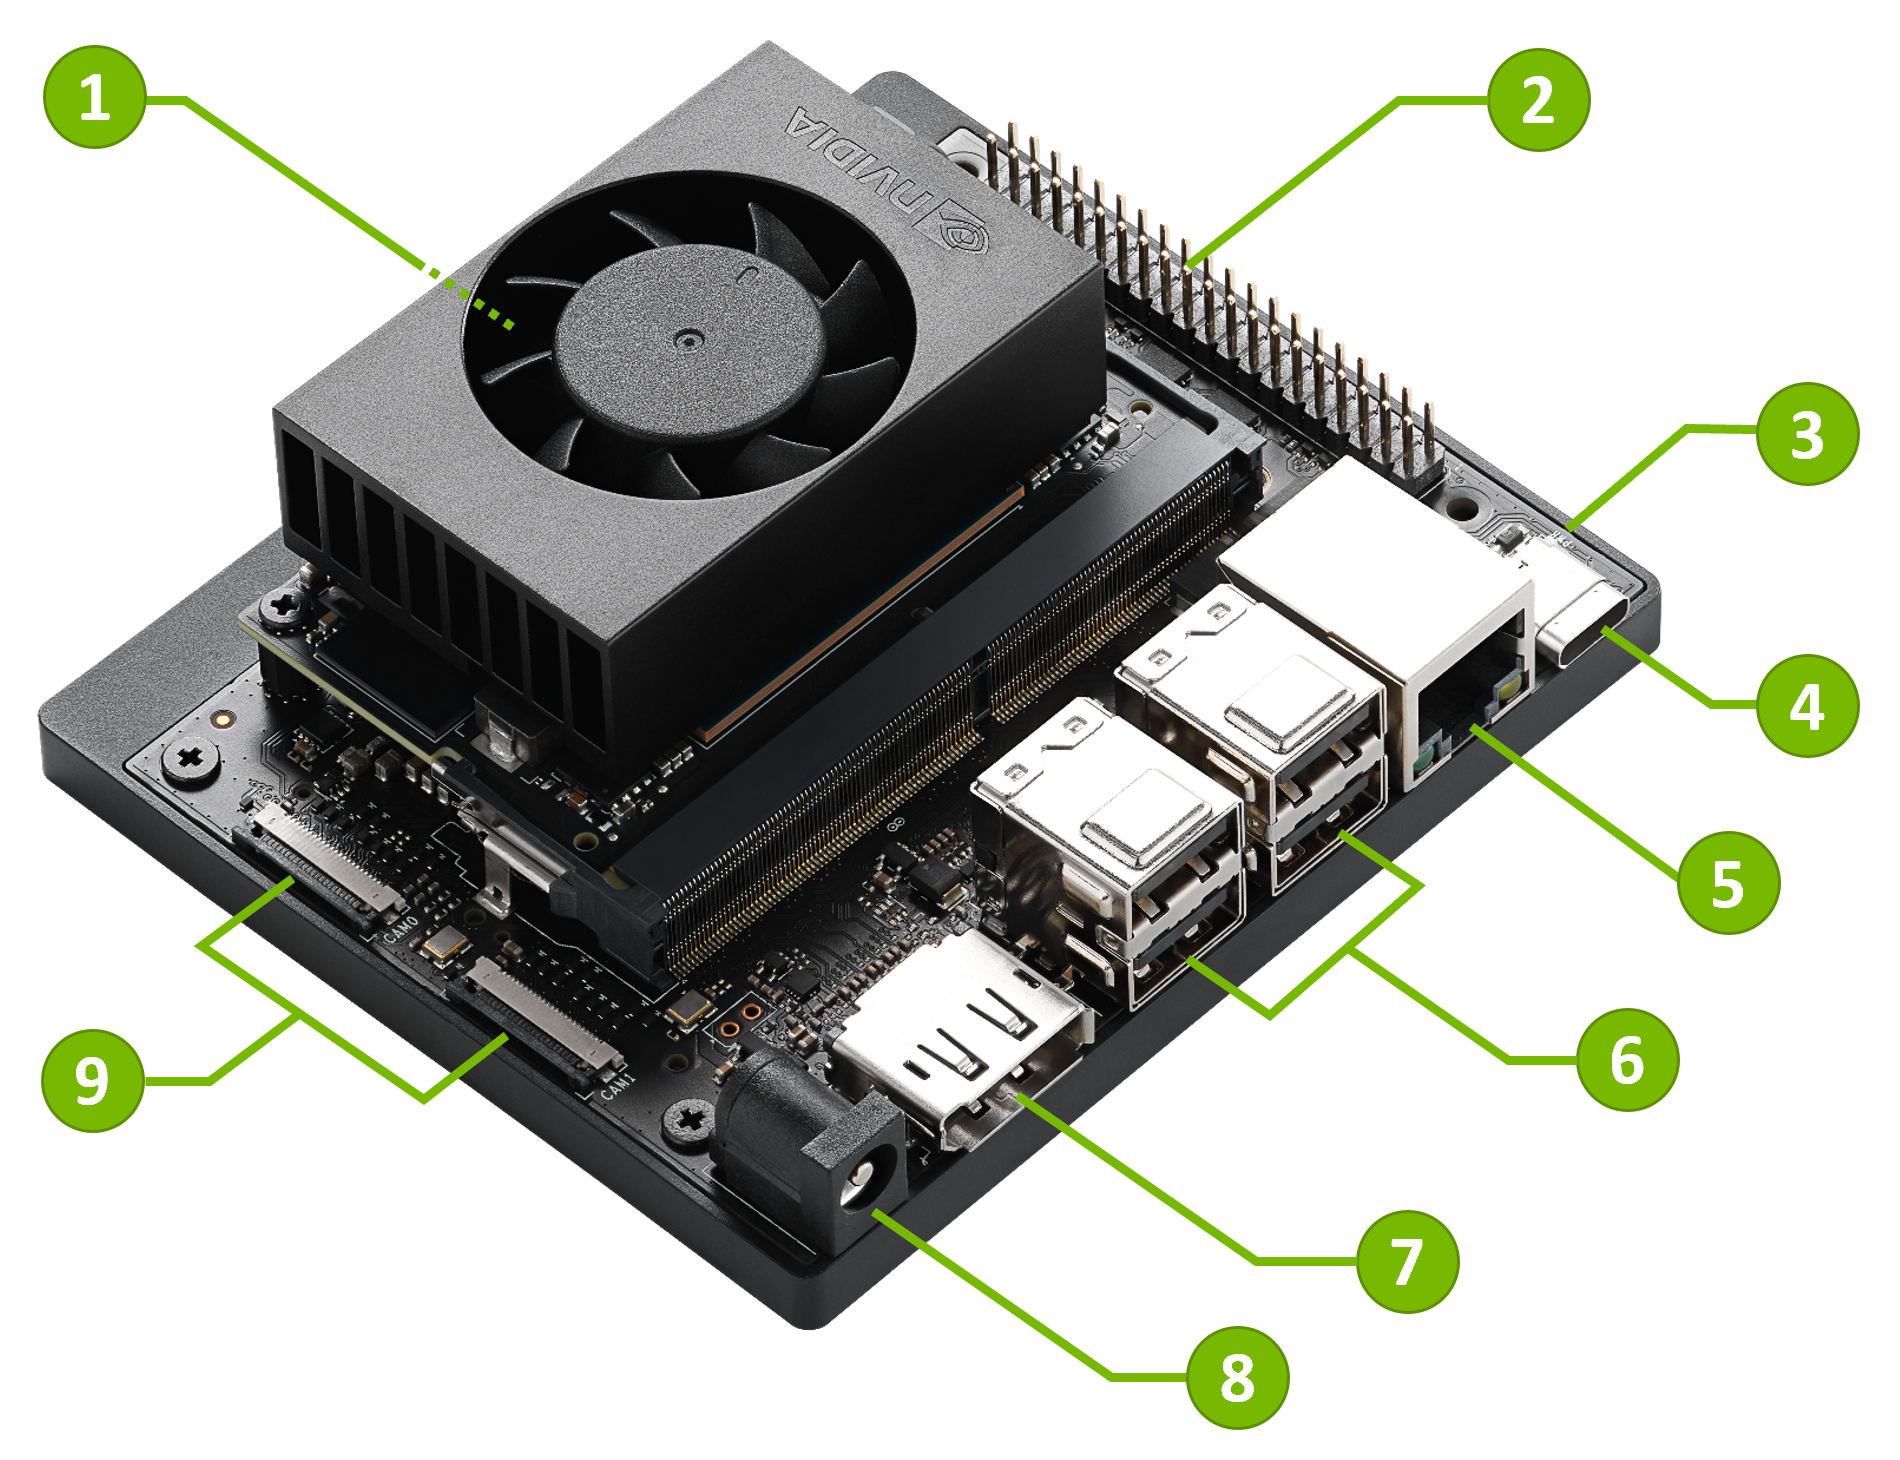
\includegraphics[width=0.8\textwidth]{jetsonOrinNano8GB.png} 

    \caption{Jetson Orin Nano Developer Kit}
\end{figure}
\begin{itemize}
    \item 1. microSD-Kartensteckplatz für den Hauptspeicher
    \item 2. 40-poliger Erweiterungsheader
    \item 3. Stromanzeigen-LED
    \item 4. USB-C-Port nur für Daten
    \item 5. Gigabit-Ethernet-Port
    \item 6. USB 3.1 Typ A Ports (x4)
    \item 7. DisplayPort-Anschluss
    \item 8. DC Barrel Jack für 19V Stromversorgung
    \item 9. MIPI CSI Kameraanschlüsse
\end{itemize}
\clearpage
\section{Technische Spezifikationen}
\subsection{Prozessor (CPU)}
\begin{itemize}
    \item \textbf{Architektur:} ARM Cortex-A78AE
    \item \textbf{Kerne:} 6 Kerne, bis zu 1,5 GHz
\end{itemize}

\subsection{Grafikprozessor (GPU)}
\begin{itemize}
    \item \textbf{Architektur:} NVIDIA Ampere, 64 Tensor Cores, 40 TOPS
\end{itemize}

\subsection{Speicher (RAM)}
\begin{itemize}
    \item 4 GB oder 8 GB LPDDR5, bis zu 68 GB/s Bandbreite
\end{itemize}

\subsection{Schnittstellen und I/O}
\begin{itemize}
    \item PCIe Gen 3 x4, USB 3.2, Gigabit-Ethernet
    \item HDMI 2.1, DP 1.2, 2x MIPI CSI-2 Kameraanschlüsse
\end{itemize}

\subsection{Leistung und Energieverbrauch}
\begin{itemize}
    \item Einstellbarer Energieverbrauch: 7 W bis 15 W
\end{itemize}

\subsection{Softwareunterstützung}
\begin{itemize}
    \item Linux for Tegra (L4T), Unterstützung für CUDA 11, C++, Python, TensorFlow, PyTorch
\end{itemize}

\section{Vergleich der Modelle}

\begin{longtable}{|l|c|c|c|}
    \hline
    \textbf{Modell} & \textbf{RAM} & \textbf{Leistung (TOPS)} & \textbf{Energieverbrauch} \\
    \hline
    Jetson Orin Nano 4GB & 4 GB & 20 TOPS & 7–15 W \\
    Jetson Orin Nano 8GB & 8 GB & 40 TOPS & 7–15 W \\
    \hline
\end{longtable}
\end{document}